\documentclass[11pt]{article}
\usepackage[utf8]{inputenc}
\usepackage[english]{babel}
\usepackage{amsmath}
\usepackage{graphicx}
\usepackage{float}
\usepackage{lipsum}
\usepackage{multicol}
\usepackage{xcolor}
\usepackage{tabularx}
\usepackage{booktabs}
\usepackage{hyperref}
\usepackage{amsfonts}
\newcolumntype{Y}{>{\centering\arraybackslash}X}
\usepackage[left=2.00cm, right=2.00cm, top=2.00cm, bottom=2.00cm]{geometry}

\title{AN2DL Reports Template}

\begin{document}

\begin{figure}[H]
    \raggedright
    \includegraphics[scale=0.5]{polimi.png} \hfill \includegraphics[scale=0.3]{airlab.jpeg}
\end{figure}

\vspace{5mm}

\begin{center}
    % Select between First and Second
    {\Large \textbf{AN2DL - Second Challenge Report}}\\
    \vspace{2mm}
    % Change with your Team Name
    {\Large \textbf{AN2DL\_C}}\\
    \vspace{2mm}
    % Team Members Information
    {\large JIALI CLAUDIO HUANG,}
    {\large YUJUE WANG,}
    {\large PENG RAO,}
    {\large LINGLI ZHANG}\\
    \vspace{2mm}
    % Codabench Nicknames
    {HUANG JIALI CLAUDIO,}
    {Yujue WANG,}
    {Peng Rao,}
    {lingli11}\\
    \vspace{2mm}
    % Matriculation Numbers
    {11032111,}
    {11047870,}
    {11022931,}
    {11022009}\\
    \vspace{5mm}
    \today
\end{center}
\vspace{5mm}

\begin{multicols}{2}
    \section{Introduction}
    Regarding this four-class image classification problem, we employs a patch-based approach where images are subdivided into smaller regions. These patches are processed using \textbf{Multiple Instance Learning (MIL)} aggregation techniques to produce a slide-level prediction.
    \section{Problem Analysis}
    The dataset consists of pathology images categorized into four subtypes: \textbf{Luminal A, Luminal B, HER2(+), and Triple negative}, includes 691 training images and their mask files.

    \begin{figure}[H]
        \centering
        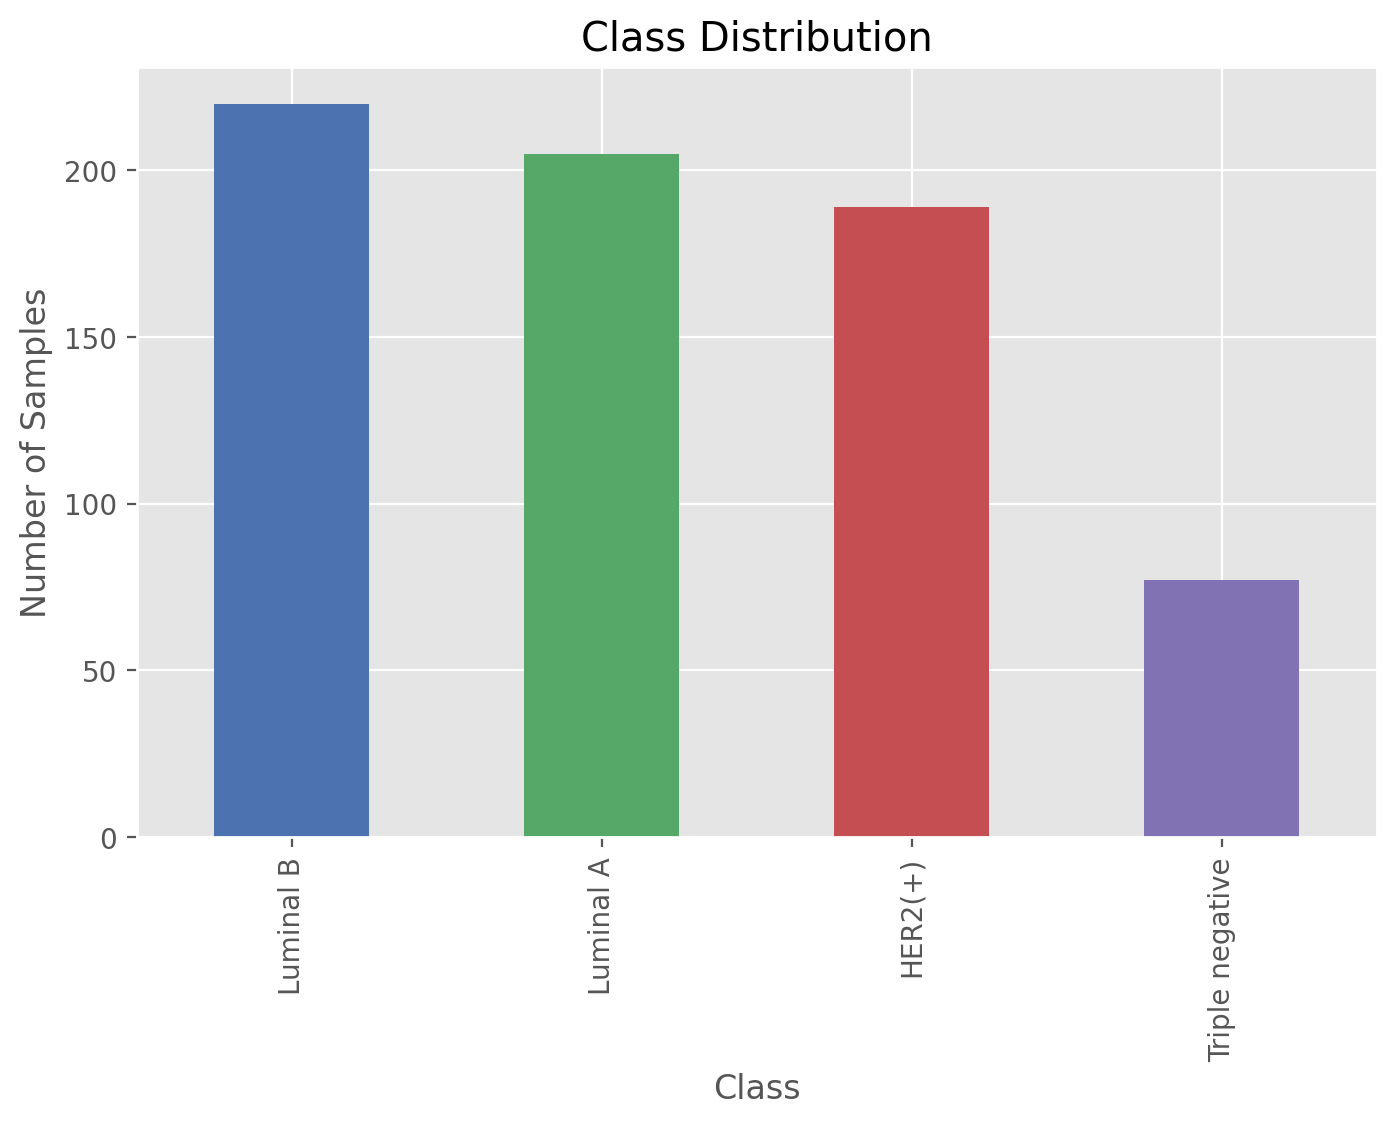
\includegraphics[width=0.75\linewidth]{class-distribution.png}
        \caption{The distribution of classes in the dataset}
    \end{figure}

    \noindent The dataset exhibits class imbalance, with the \textbf{Luminal B} subtype being the most prevalent, \textbf{Triple negative} subtypes are underrepresented.

    We extract multiple patches from a pathology image.

    \begin{figure}[H]
        \centering
        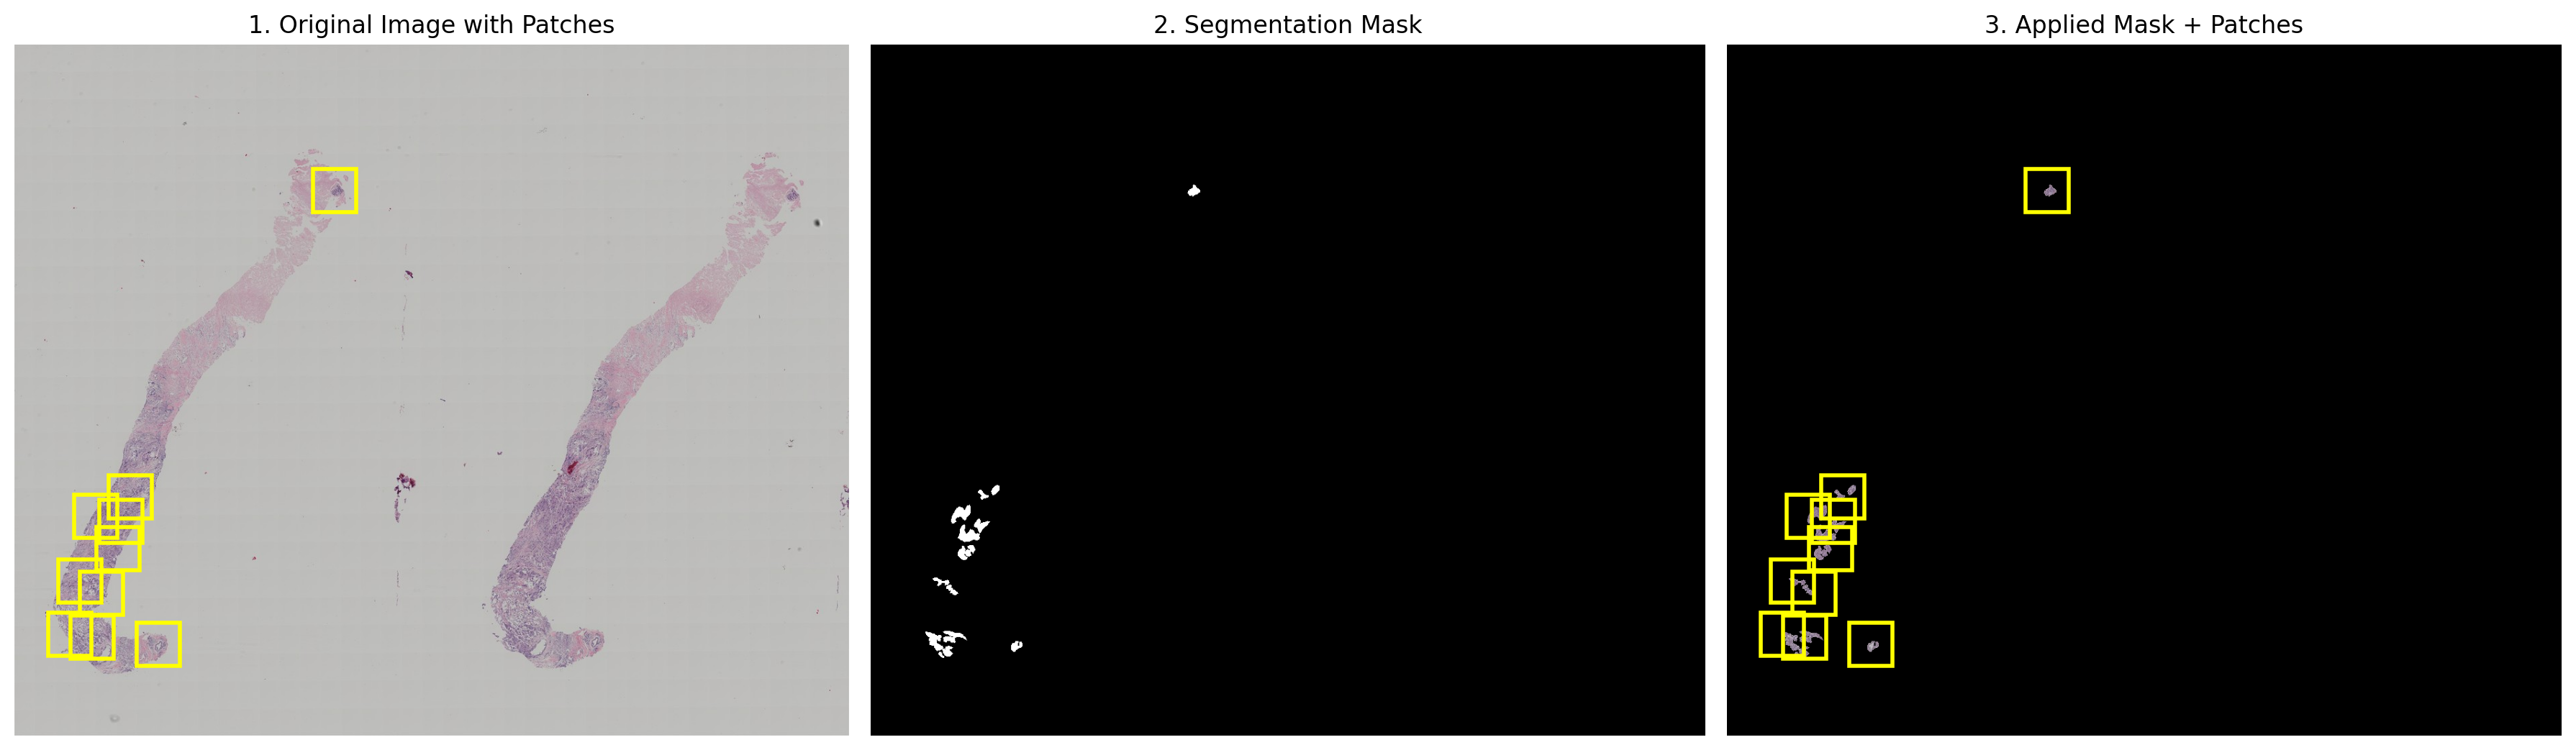
\includegraphics[width=1.0\linewidth]{patches_example1.png}
        \caption{Example of extracted patches from a pathology image (0000)}
    \end{figure}

    \begin{figure}[H]
        \centering
        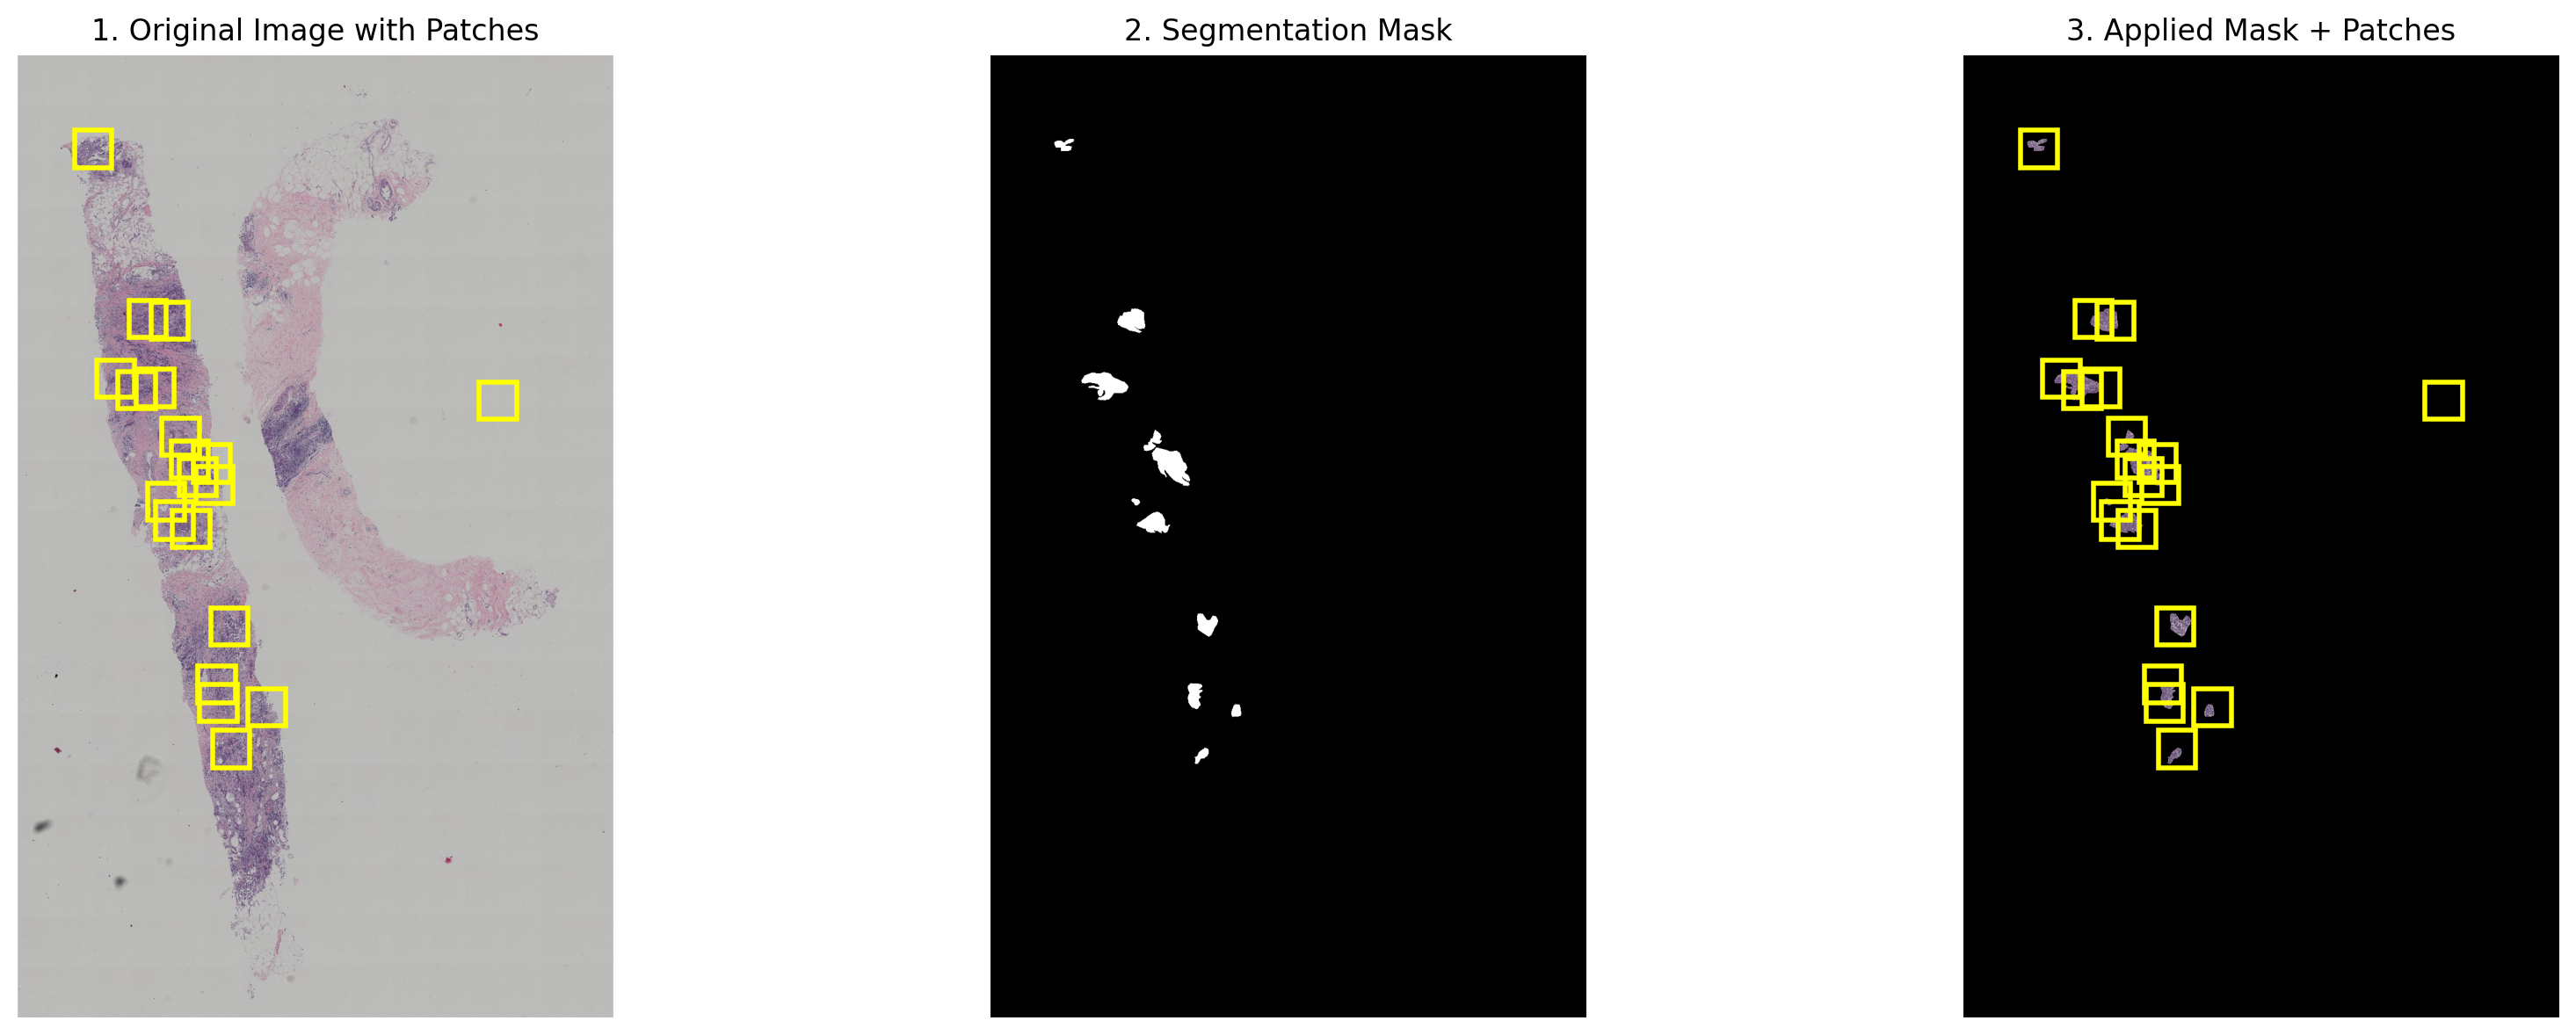
\includegraphics[width=1.0\linewidth]{patches_example2.png}
        \caption{Example of extracted patches from a pathology image (0002)}
    \end{figure}

    \section{Method}
    \subsection{Noisy image recognition}
    We observed that some images in the dataset are noisy or corrupted (Orcs and Slime), which can negatively impact model performance. To address this, we used two layers of defense:
    \begin{itemize}
        \item \textbf{Color Check}: Histology images are never green. If an image has significant green pixels (common for orcs/slimes), it is immediately trashed.
        \item \textbf{CLIP Classification}: Use \textbf{openai/clip-vit-large-patch14} to identify and filter out these noisy images from the training set. We create text prompts like "a histology image" and "a green slime histology image" to classify images. If an image is classified as "green slime histology image" with high confidence, it is marked as noisy.
    \end{itemize}
    Finally, we removed \textbf{101} noisy images from the training set, get \textbf{590} clean images for training.

    \subsection{Data Augmentation}
    To enhance model robustness and generalization, we applied various data augmentation techniques during training, including
    \begin{itemize}
        \item Random rotations and flips
        \item Color jittering (brightness, contrast, saturation adjustments)
        \item Mixup augmentation
    \end{itemize}

    \subsection{Dual-stream MIL Network}
    We use a Dual-Stream Multiple Instance Learning (MIL) architecture ~\cite{li_dual-stream_2021} designed to integrate local morphological details with global spatial context. As illustrated in ~\ref{fig:dual_stream_mil}, the network processes a image through two parallel streams: a \textit{Local Stream} (Bag of Instances) and a \textit{Global Stream} (Contextual View), fusing their representations for final classification.

    \begin{figure}[H]
        \centering
        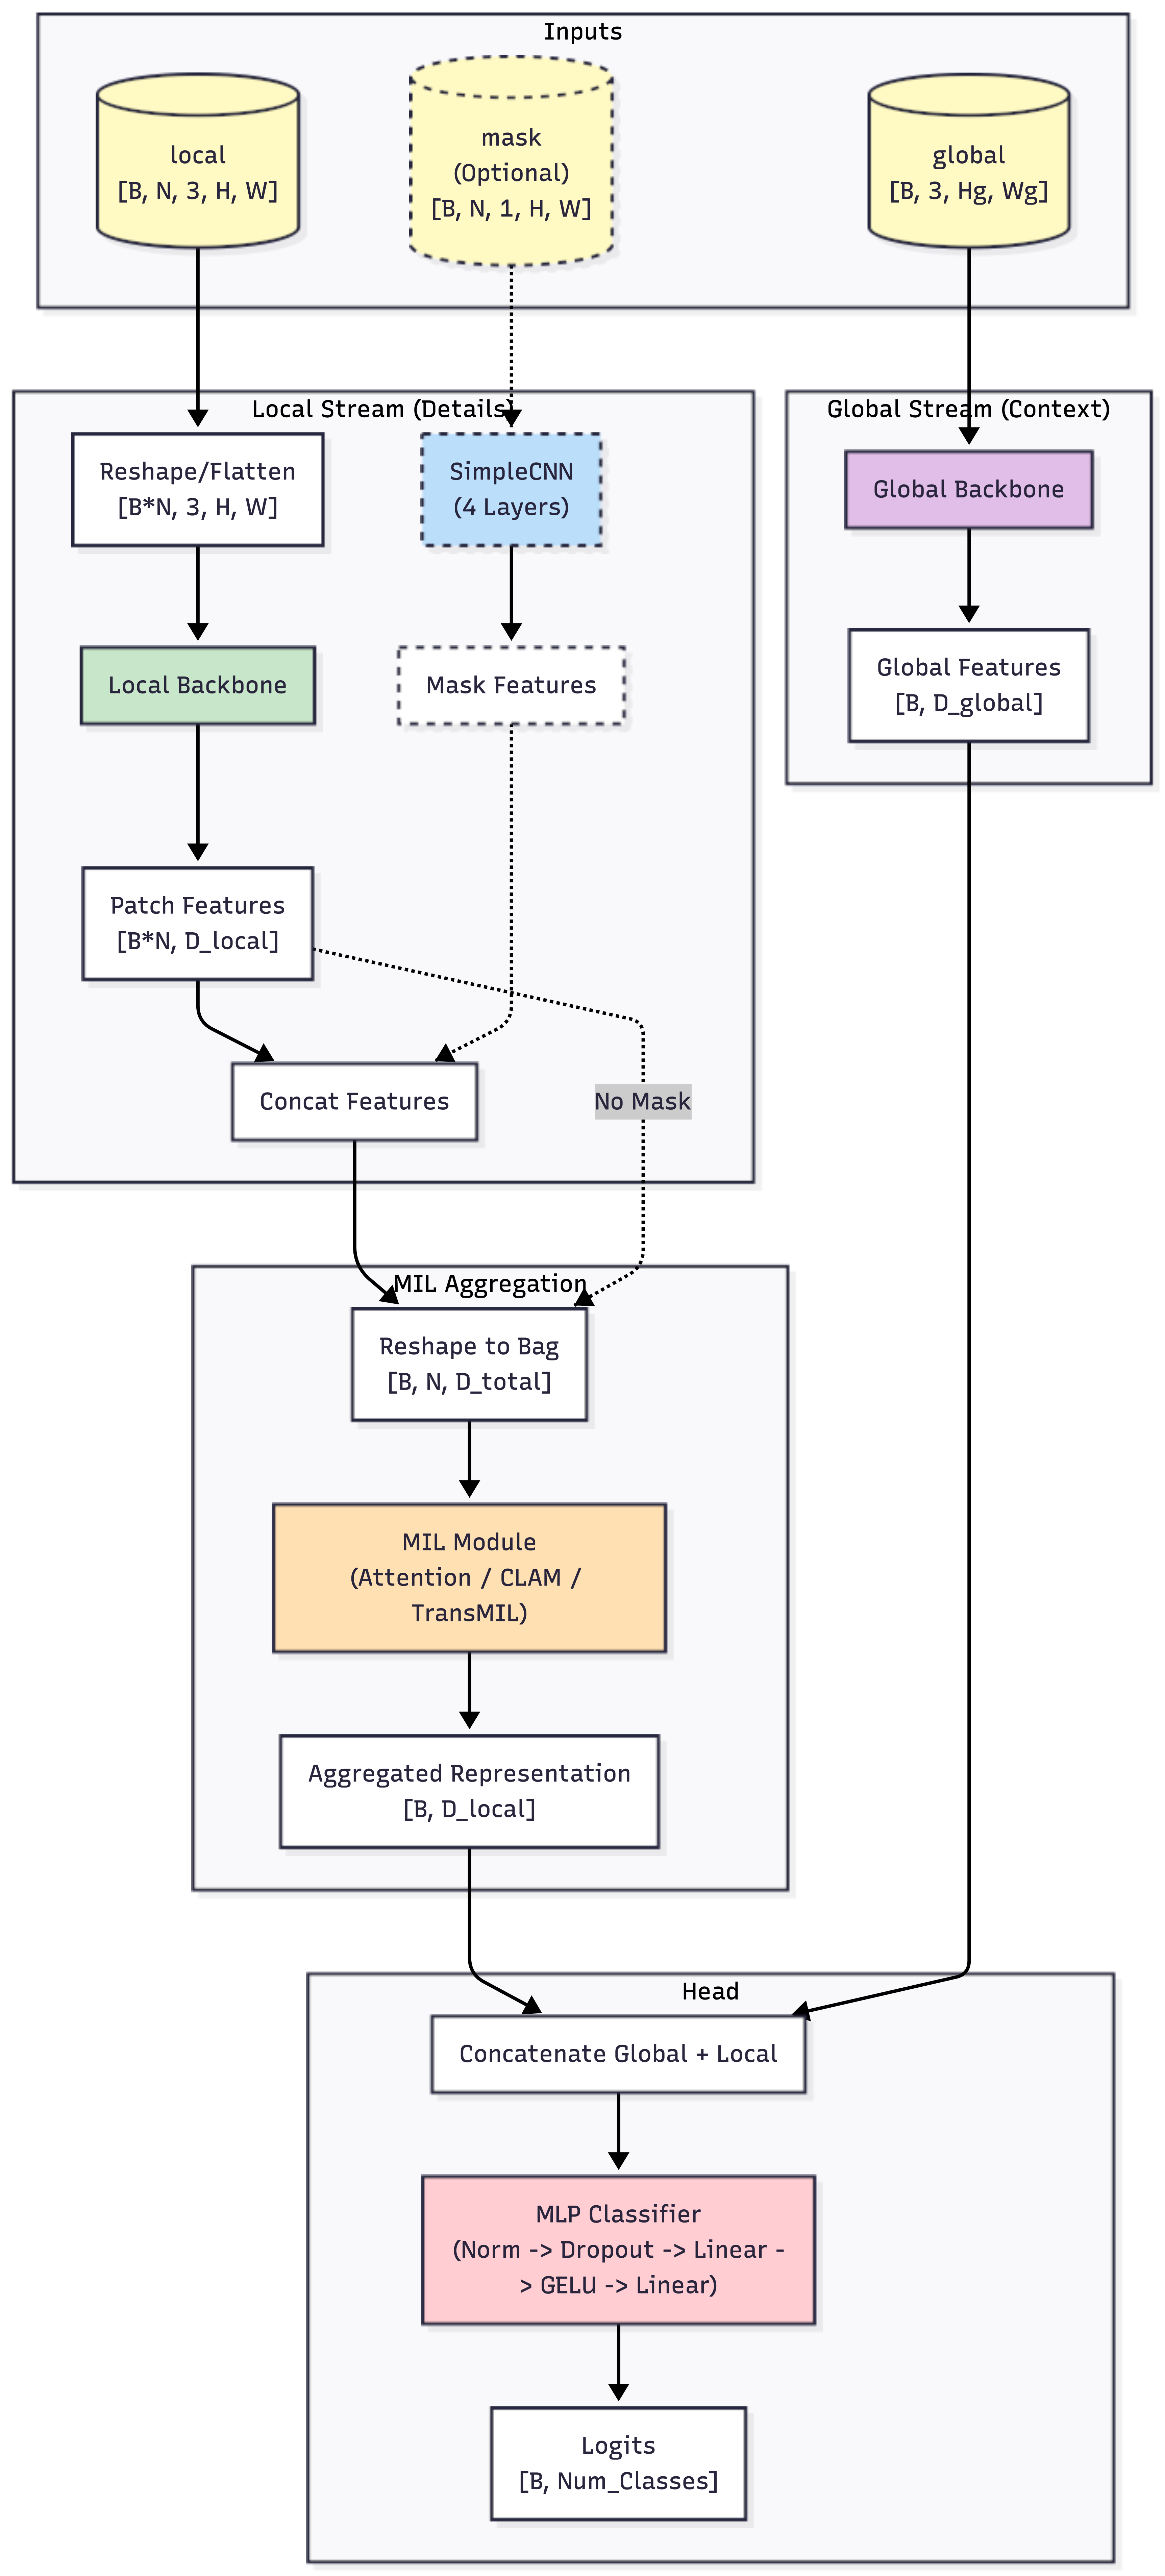
\includegraphics[height=0.5\textheight]{Dual-Stream-MIL.png}
        \caption{Dual-Stream MIL Architecture}
        \label{fig:dual_stream_mil}
    \end{figure}

    \paragraph{Local Stream}
    The local stream processes individual patches extracted from the image. Each patch is passed through a shared backbone network (ResNet34) to extract feature representations. These features are then projected into a lower-dimensional space via a bottleneck layer.

    \paragraph{Optional Mask Fusion}
    Since the binary mask is provided, we experimented with fusing mask information into the patch features.

    \paragraph{MIL Aggregation}
    To obtain a permutation-invariant representation of the entire bag, we employ an aggregation function.

    \paragraph{Global Stream}
    To capture macro-architectural patterns often lost in patch-based tiling, we introduce a global stream. A downsampled view of the image is processed by a secondary backbone (ResNet18). Similar to the local stream, this is projected via a bottleneck.
    \pagebreak

    \section{Experiments}
    We conducted extensive experiments to evaluate the performance of our proposed Dual-Stream MIL model. The experiments were designed to assess the impact of various components, including the use of mask information, different aggregation methods, and data augmentation techniques.
    \paragraph{Patch Extraction}
    We extracted patches of size 224x224 pixels from each image using a stride of 112 pixels. Patches with less than 50\% tissue content were discarded based on the provided binary masks. To avoid class imbalance, we ensured that each bag contained a balanced number of patches from each class using WeightedRandomSampler.
    \paragraph{Optimizer}
    We used the AdamW optimizer with a learning rate of 1e-4 and weight decay of 1e-2. We also expored the Lion optimizer.


    \begin{table}[H]
        \centering
        \setlength{\tabcolsep}{3pt}
        \caption{Experimental measurements for different models.}
        \begin{tabularx}{\linewidth}{lY}
            \toprule
            Model(local + global)             & F1-score in validation \\
            \midrule
            resnet18+resnet18                 & 0.3674                 \\
            efficientnet\_b0+efficientnet\_b0 & 0.3734                 \\

            densenet121+resnet18              & 0.3828                 \\
            resnet18+convnext\_tiny           & 0.3482                 \\
            \textbf{convnext\_tiny+resnet18}  & \textbf{0.4226}        \\
            resnet50+resnet18                 & 0.3116                 \\
            \bottomrule
        \end{tabularx}
        \label{tb:Measurements}
    \end{table}

    \section{Discussion}


    \section{Suggest improvements}



    \bibliography{references}
    \bibliographystyle{abbrv}

\end{multicols}
\end{document}